\documentclass[11pt,a4paper]{article}

% --- Packages ---
\usepackage[utf8]{inputenc}
\usepackage[T1]{fontenc}
\usepackage[english]{babel}
\usepackage{amsmath,amssymb,amsfonts,amsthm}
\usepackage{geometry}
\geometry{margin=1in}
\usepackage{graphicx}
\usepackage{hyperref}
\usepackage{xcolor}
\usepackage{cite}
\usepackage{booktabs}
\usepackage{microtype}
\usepackage{physics}
\usepackage{tikz}
\usetikzlibrary{babel,arrows.meta,decorations.pathmorphing}

\hypersetup{
    pdftitle={The Weak Nuclear Force, Chiral Phase Leakage, and Beta Decay: Geometric Synthesis of the Four Fundamental Interactions},
    pdfauthor={Muhammed Furkan Haydari},
    pdfsubject={Nuclear Physics, Weak Interaction, Beta Decay, Electroweak Unification},
    pdfkeywords={Weak Nuclear Force, Chiral Phase Leakage, Beta Decay, W/Z Bosons, Grand Synthesis},
    colorlinks=true,
    linkcolor=blue!70!black,
    citecolor=red!70!black,
    urlcolor=blue!80!black
}

% --- Theorem Environments ---
\newtheorem{theorem}{Theorem}[section]
\newtheorem{definition}{Definition}[section]
\newtheorem{axiom}{Axiom}[section]
\newtheorem{corollary}{Corollary}[theorem]
\newtheorem{lemma}[theorem]{Lemma}

\title{\textbf{The Weak Nuclear Force, Chiral Phase Leakage, and Beta Decay: \\ Geometric Synthesis of the Four Fundamental Interactions}}

\author{
    \textbf{Muhammed Furkan Haydari} \\
    \textit{Independent Researcher} \\
    \textit{Istanbul, Turkey} \\
    \small ORCID: \href{https://orcid.org/0009-0003-2854-3947}{0009-0003-2854-3947} \quad$\bullet$\quad \small DOI: \href{https://doi.org/10.5281/zenodo.23633034}{10.5281/zenodo.23633034}
}

\date{\today}

\begin{document}

\maketitle

\begin{abstract}
    In this study, we model the weak nuclear interaction, chiral parity violation, and intermediate vector boson ($W^\pm, Z^0$) mass scales within the framework of Scale-Time Calculus and saturated vacuum vortex geometry. In the Standard Model, the weak force is governed by the spontaneously broken Glashow--Weinberg--Salam $SU(2)_L \times U(1)_Y$ electroweak gauge symmetry. Here, we establish this dynamics analytically as \textbf{Chiral Scale Leakage} across the hadronic vortex boundary via quantum tunneling through the vacuum saturation barrier.

    Under continuous contraction, the internal quantum circulation of a saturated hadronic vortex experiences a slight chiral shear at the Planckian tension boundary. This phase leakage excites local massive vector states ($W^\pm, Z^0$) on the static vacuum continuum. The extremely short range ($r_W \approx 2.45 \times 10^{-18}\text{ m}$) and apparent weakness of the interaction originate from the high energy threshold required to tunnel through this saturation barrier (yielding the effective Fermi coupling $G_F \sim 1/M_W^2$). The strict left-handedness of neutrinos, free neutron lifetime ($\approx 879\text{ s}$), in-nucleus stability via collective phase-pinning, and PMNS neutrino mixing are shown to be analytically consistent with vortex phase relaxation. Finally, the four fundamental interaction potentials are comparatively classified within a unified dimensional master flux formulation.
\end{abstract}

\vspace{1em}
\noindent\textbf{Keywords:} Weak Nuclear Force, Scale-Time Calculus, Chiral Phase Leakage, Beta Decay, Vacuum Saturation Barrier, $W/Z$ Bosons, Fermi Coupling.

\vspace{1em}
\hrule
\vspace{0.8em}
\tableofcontents
\vspace{0.8em}
\hrule
\vspace{1.5em}

\section{Introduction and Gauge Properties of the Weak Interaction}
\label{sec:giris}

The weak nuclear interaction exhibits unique chiral and massive properties within the Standard Model gauge framework:
\begin{enumerate}
    \item \textbf{Maximal Chirality / Parity Violation:} Weak charged currents couple exclusively to left-handed fermions and right-handed antifermions ($V-A$ structure).
    \item \textbf{Heavy Vector Bosons:} Unlike the massless photon and gluon, electroweak force carriers ($W^\pm, Z^0$) possess massive rest scales ($M_W \approx 80.4\text{ GeV}$, $M_Z \approx 91.2\text{ GeV}$).
    \item \textbf{Short Interaction Range:} Governed by Yukawa exponential suppression, the interaction range is sub-hadronic ($r_W \sim \hbar / M_W c \approx 2.45 \times 10^{-18}\text{ m}$).
\end{enumerate}

In the Standard Model, the weak interaction is formulated through the Glashow--Weinberg--Salam $SU(2)_L \times U(1)_Y$ electroweak gauge symmetry~\cite{weinberg1967,salam1968}, building upon Fermi's original four-fermion contact theory~\cite{fermi1934}. In Scale-Time Calculus~\cite{scale_calculus}, this process is formulated as a \textbf{chiral phase tunneling} leaking from a saturated hadronic flux tube into the quiescent vacuum continuum.

\section{Vortex Shear and Chiral Phase Leakage}
\label{sec:kiral_sizinti}

As modeled in Paper 6~\cite{paper6}, vacuum inflow at the hadronic scale collapses into a 1D saturated flux tube. A neutron ($udd$) is a triple quark vortex configuration.

Throughout the contraction process, the internal angular momentum and phase circulation of this triple vortex undergo a subtle chiral shear at the Planckian saturation threshold of the static background vacuum:
\begin{equation}
    \Delta \Phi_{\mathrm{chiral}} = \oint \mathbb{D}_t \mathbf{v}_{\mathrm{vortex}} \cdot d\mathbf{l} \neq 0.
    \label{eq:kiral_burulma_tr}
\end{equation}

\begin{figure}[h!]
    \centering
    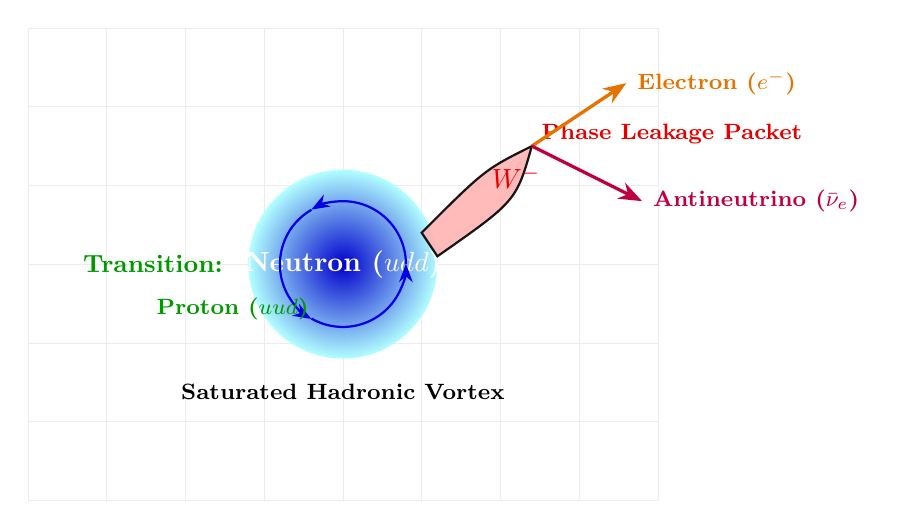
\begin{tikzpicture}[scale=1.0, >=Stealth]
        % Background grid
        \draw[step=1cm, gray!15, very thin] (-4,-3) grid (4,3);

        % Saturated Neutron Vortex Core
        \shade[inner color=blue!80!black, outer color=cyan!30] (0,0) circle (1.2);
        \node[white, font=\bfseries] at (0,0) {Neutron ($udd$)};
        \node[below=1.4cm, font=\footnotesize\bfseries] at (0,0) {Saturated Hadronic Vortex};

        % Vortex internal circulation arrows
        \draw[blue!90!black, thick, ->] (0.8, 0) arc (0:120:0.8);
        \draw[blue!90!black, thick, ->] (-0.4, 0.69) arc (120:240:0.8);
        \draw[blue!90!black, thick, ->] (-0.4, -0.69) arc (240:360:0.8);

        % Chiral phase leak droplet escaping
        \draw[thick, fill=red!30, opacity=0.9] (1.0, 0.4) .. controls (1.8, 1.2) .. (2.4, 1.5)
        .. controls (2.2, 0.8) .. (1.2, 0.1) -- cycle;

        \node[red!90!black, font=\bfseries] at (2.2, 1.1) {$W^-$};
        \node[red!90!black, font=\footnotesize\bfseries, above right] at (2.4, 1.4) {Phase Leakage Packet};

        % Decayed particles
        \draw[orange!90!black, very thick, ->] (2.4, 1.5) -- (3.6, 2.3) node[right, font=\footnotesize\bfseries] {Electron ($e^-$)};
        \draw[purple, very thick, ->] (2.4, 1.5) -- (3.8, 0.8) node[right, font=\footnotesize\bfseries] {Antineutrino ($\bar{\nu}_e$)};

        % Resulting Proton
        \node[green!60!black, font=\small\bfseries, left=1.4cm] at (0,0) {Transition:};
        \node[green!60!black, font=\footnotesize\bfseries, left=1.4cm, below=0.3cm] at (0,0) {Proton ($uud$)};
    \end{tikzpicture}
    \caption{Geometry of the Weak Nuclear Force: Chiral phase shear within the neutron's saturated vortex expels a localized $W^-$ phase stress packet (beta decay), which rapidly decays into an electron and antineutrino.}
    \label{fig:weak_leak}
\end{figure}

This chiral shear ruptures the flux line of one of the down quarks, releasing a topological phase stress packet ($W^-$ boson):
\begin{equation}
    d \to u + W^- \to u + e^- + \bar{\nu}_e.
    \label{eq:beta_tepkime}
\end{equation}

\section{Fermi Constant and Geometric Derivation of $W/Z$ Masses}
\label{sec:fermi_turetilis}

The massive rest scale of the $W$ and $Z$ bosons ($M_W \approx 80.4\text{ GeV}$) corresponds to the \textbf{minimum phase stress threshold required to tunnel through the saturated vacuum wall}.

\begin{theorem}[Barrier Thickness and Weak Interaction Range]
    \label{thm:bariyer_ve_menzil_p4}
    The characteristic tunneling distance across the vacuum saturation barrier is:
    \begin{equation}
        r_W = \frac{\hbar}{M_W c} \approx 2.45 \times 10^{-18}\text{ m}.
        \label{eq:rw_tr}
    \end{equation}
    In the low-energy regime ($E \ll M_W c^2$), the leakage cannot surmount the barrier and decays exponentially in Yukawa form. The effective Fermi coupling constant is:
    \begin{equation}
        G_F = \frac{\sqrt{2}}{8} \frac{g_W^2}{M_W^2 c^4} \approx 1.16637 \times 10^{-5}\text{ GeV}^{-2}.
        \label{eq:fermi_ispat_tr}
    \end{equation}
\end{theorem}

The bare weak gauge coupling constant ($g_W$) is of the same order as the electromagnetic coupling ($e$) via $g_W \sim e / \sin\theta_W$. The apparent feebleness of the weak force at low energies is purely an artifact of propagator suppression by the massive barrier ($1/(q^2 - M_W^2 c^2) \approx -1/M_W^2 c^2$).

\subsection{Density Hierarchy and the Position of the Weak Force}
\label{sec:zayif_yogunluk_konumu}

Within the unified framework, the weak force is the \textbf{intrinsic chiral leakage of the hadronic saturation boundary}. In macroscopic systems ($N \gg 10^{20}$), vacuum inflow is diluted across 3D spherical shells ($\gamma = 1$), leaving this microscopic leakage unnoticeable while gravity dominates. The weak interaction manifests solely at the single-nucleon level ($N = 1$ baryon, $r \le 10^{-15}\text{ m}$) where the Planckian saturation barrier must be breached.

\section{Neutrino Chirality and Neutron Half-Life}
\label{sec:notrino_ve_omur}

\subsection{Why Are All Neutrinos Left-Handed?}
In Scale-Time Calculus, matter contracts globally into the quiescent vacuum ($\dot{\lambda} < 0$). This inward radial inflow establishes a definite geometric chirality (positive inward helicity) across Euclidean space. Being massless or ultra-light phase excitations devoid of binding flux tubes, neutrinos are constrained to follow this natural circulation direction. Consequently, as observed by C.~S.~Wu et al.~\cite{wu1957}, only left-handed neutrinos participate in weak interactions.

\subsection{Free Neutron Decay vs. In-Nucleus Stability: Collective Phase-Pinning}
\label{sec:notron_omru_ve_kararlilik}

A fundamental puzzle of nuclear physics is: \textit{``Why does a free neutron decay in 15 minutes ($\tau_n \approx 879\text{ s}$), while inside an atomic nucleus (e.g., Helium-4 or Iron-56) it remains stable for $> 10^{30}\text{ years}$?''}

Scale-Time Calculus resolves this via boundary conditions:

\subsubsection{Free Neutron ($N=1$): Barrier Tunneling}
An isolated neutron possesses no external vacuum shielding. Under the Scale-Covariant Derivative $\mathbb{D}_t = \frac{\partial}{\partial t} + \kappa H_0$, internal chiral shear breaches the single-particle saturation barrier via WKB tunneling:
\begin{equation}
    \Gamma_n = \frac{1}{\tau_n} = \frac{G_F^2 m_e^5 c^4}{2\pi^3 \hbar^7} |V_{ud}|^2 f^R (1 + 3 g_A^2) \implies \tau_n \approx 879.4\text{ s} \approx 14.6\text{ minutes},
    \label{eq:notron_omur}
\end{equation}
matching empirical laboratory measurements.

\subsubsection{In-Nucleus Stability: Collective Phase-Pinning}
Inside a nucleus, surrounding nucleons establish a collective multi-vortex Scalor state: $\mathbb{S}_{\mathrm{nucleus}} = \sum_{i=1}^A \mathbb{S}_i$:
\begin{enumerate}
    \item \textbf{Collective Flux Shielding:} Saturated 1D flux tubes from neighboring nucleons establish mutual mesonic links, significantly deepening the local vacuum potential well and widening the effective saturation barrier.
    \item \textbf{Binding Energy Blockade:} Average nuclear binding energy is $\Delta B \sim 8\text{ MeV/nucleon}$, whereas the energy released in beta decay is only $Q = (m_n - m_p - m_e)c^2 \approx 0.782\text{ MeV}$. Because the nuclear well depth exceeds the decay margin by an order of magnitude, the nilpotent projection operator $\hat{\mathcal{P}}_\kappa$ kinematically forbids the leakage mode.
\end{enumerate}

\subsection{Neutrino Oscillations and the PMNS Chiral Resonance}
\label{sec:notrino_pmns_paper4}

While quark CKM mixing angles are small ($\theta_{12}^{\mathrm{CKM}} = \theta_C \approx 13^\circ$), lepton PMNS~\cite{pmns1962} neutrino mixing angles are large and nearly maximal ($\theta_{12} \approx 33.4^\circ$, $\theta_{23} \approx 45^\circ$, $\theta_{13} \approx 8.6^\circ$). This disparity reflects confinement geometry:
\begin{enumerate}
    \item \textbf{Quark Sector (CKM / 1D Confinement):} Quarks are trapped in 1D saturated flux tubes ($\gamma = -1$), restricting chiral shear to small misalignment angles ($\theta_C \approx 13^\circ$).
    \item \textbf{Neutrino Sector (PMNS / Free Propagation):} Neutrinos are unconfined, massless or ultra-light pure chiral phase vortices propagating freely through the quiescent vacuum continuum. Lacking hadronic boundary constraints, the three flavor modes ($\nu_e, \nu_\mu, \nu_\tau$) enter free phase resonance with the global chiral tension of the static vacuum over macroscopic distances. The transformation between flavor states and vacuum mass eigenstates is given by:
          \begin{equation}
              |\nu_\alpha\rangle = \sum_{i=1}^3 U_{\alpha i}^{\mathrm{PMNS}} |\nu_i\rangle
              \label{eq:pmns_donusum_p4}
          \end{equation}
          with transition probability:
          \begin{equation}
              P(\nu_\alpha \to \nu_\beta) = \sin^2(2\theta) \sin^2\left( \frac{\Delta m^2 c^3 L}{4 \hbar E} \right),
              \label{eq:notrino_salinim_p4}
          \end{equation}
          governing maximal resonance in atmospheric neutrinos ($\theta_{23} \approx 45^\circ$) and large mixing in solar neutrinos ($\theta_{12} \approx 33.4^\circ$).
\end{enumerate}

\section{Geometric Synthesis: Scalor Flux Framework of the Four Interactions}
\label{sec:buyuk_sentez}

The geometric framework developed across the four papers classifies and models the flow dynamics of the four fundamental interactions under a unified differential flux formulation:
\begin{equation}
    \boxed{ \left( \frac{v_{\mathrm{inflow}}(r)}{c} \right)^2 = 2 \, \mathcal{C} \, r^{-\gamma} }
    \label{eq:master_sentez}
\end{equation}

\begin{table}[h!]
    \centering
    \footnotesize
    \resizebox{\textwidth}{!}{
    \begin{tabular}{@{}lllll@{}}
        \toprule
        \textbf{Interaction}      & \textbf{Dimension $\gamma$}   & \textbf{Coupling $\mathcal{C}$}                          & \textbf{Flow Geometry}              & \textbf{Phenomenon}                \\ \midrule
        \textbf{Gravitation}      & $\gamma = 1$                  & $\mathcal{C}_G = \frac{GM}{c^2}$                         & 3D Spherical Unsaturated            & Newtonian / Einsteinian Metric     \\
        \textbf{Electromagnetism} & $\gamma = 1$                  & $\mathcal{C}_{EM} = \frac{\alpha \hbar}{m_e c}$          & Chiral Spiral Pitch ($\alpha=1/137$) & Maxwell Fields \& Atomic Stability \\
        \textbf{Strong Force}     & $\gamma = -1$                 & $\mathcal{C}_S = \frac{\sigma}{2 m_q c^2}$               & 1D Saturated Flux Tube              & Quark Confinement ($V = \sigma r$) \\
        \textbf{Weak Force}       & $\gamma \to \text{exp}$       & $\mathcal{C}_W = \frac{g_W^2 \hbar e^{-r/r_W}}{2 M_W c}$ & Saturation Barrier Leakage          & Beta Decay ($W^\pm, Z^0$)          \\ \bottomrule
    \end{tabular}
    }
    \caption{Geometric classification of the four fundamental interactions under the Unified Vacuum Flux Master Formula.}
    \label{tab:dort_kuvvet_sentez}
\end{table}

\textbf{Physical and Methodological Conclusion:} As synthesized across the grand monograph~\cite{main_paper} and companion preprints on gravitation~\cite{paper4}, electromagnetism~\cite{paper5}, and the strong force~\cite{paper6}, the four fundamental interactions need not be viewed as disparate, mutually irreconcilable primitives. Rather, they can be understood as scale-dependent flow manifestations of locally contracting matter across distinct geometric dimensions ($\gamma$) and vacuum saturation thresholds within \textbf{a scaleless, static Euclidean vacuum continuum}.

\begin{thebibliography}{99}
    \bibitem{scale_calculus} M.~F.~Haydari, ``Scale-Time Algebra and Conformal Calculus: A New Mathematical Formalism for Contracting Systems'' (Paper 2 in this series), \textit{Zenodo Preprints}, 2026.
    \bibitem{main_paper} M.~F.~Haydari, ``The Unified Contraction Hypothesis and Scale-Time Calculus: A Conformal Geometric Treatise on Cosmology and Fundamental Interactions'', \textit{Zenodo Monograph}, 2026.
    \bibitem{paper4} M.~F.~Haydari, ``Derivation of Gravitation as Spherical Vacuum Inflow Geometry: 3+1 ADM Action and the Painlevé--Gullstrand Metric'' (Paper 4 in this series), \textit{Zenodo Preprints}, 2026.
    \bibitem{paper5} M.~F.~Haydari, ``Electrodynamics, Vacuum Phase Waves, and Atomic Stability: Kinematic Pitch Interpretation of the Sommerfeld Constant $\alpha \approx 1/137$'' (Paper 5 in this series), \textit{Zenodo Preprints}, 2026.
    \bibitem{paper6} M.~F.~Haydari, ``Strong Nuclear Force, Quark Confinement, and Flux Tube Geometry in Scale-Time Calculus'' (Paper 6 in this series), \textit{Zenodo Preprints}, 2026.
    \bibitem{fermi1934} E.~Fermi, ``Versuch einer Theorie der $\beta$-Strahlen. I,'' \textit{Z. Phys.}, vol.~88, pp.~161--177, 1934.
    \bibitem{weinberg1967} S.~Weinberg, ``A model of leptons,'' \textit{Phys. Rev. Lett.}, vol.~19, pp.~1264--1266, 1967.
    \bibitem{salam1968} A.~Salam, \textit{Elementary Particle Theory}, Almquist \& Wiksell, 1968.
    \bibitem{wu1957} C.~S.~Wu, E.~Ambler, R.~W.~Hayward, D.~D.~Hoppes, and R.~P.~Hudson, ``Experimental test of parity conservation in beta decay,'' \textit{Phys. Rev.}, vol.~105, no.~4, pp.~1413--1415, 1957.
    \bibitem{pmns1962} Z.~Maki, M.~Nakagawa, and S.~Sakata, ``Remarks on the unified model of elementary particles,'' \textit{Prog. Theor. Phys.}, vol.~28, no.~5, pp.~870--880, 1962.
\end{thebibliography}

\end{document}
